\documentclass{school-22.211-notes}
\date{March  7, 2012}

\begin{document}
\maketitle

%%%%%%%%%%%%%%%%%%%%%%%%% Resonance Models Day 6 %%%%%%%%%%%%%%%%%%%%%%%%%%%%
\lecture{Intro to 2D Transport: Three Methods for Solving Pin Cell Problems}
This section was given 03/11/2013 and 03/13/2013 in 22.212. The purpose of this section is to generate $P_{FF}$, and from there compute energy shape of flux and/or Bell factor. Basic steps: 
\begin{enumerate}
\item Compute $P_{FF}$. For instance, for 1D infinite slab, $P_{FF} = 1 - P_{\mathrm{escape}}$. 

\item From $P_{FF}$ compute \hi{spatially averaged energy shape}: 
\eqn{ \Aboxed{f_F(\mu) &= P_{FF} \frac{\Sigma_{pot}^F}{\Sigma_t^F} + P_{FM}}  & 
  \Aboxed{f_M(\mu) &= P_{MM} + P_{FM} \frac{\Sigma_{pot}^F V_F}{\Sigma^M V_M} } }
\begin{figure}[h]
  \centering
  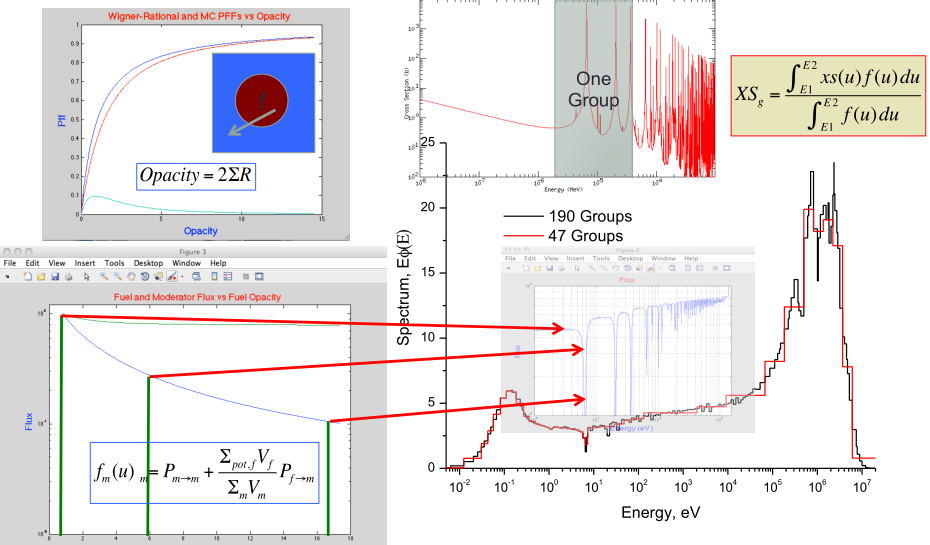
\includegraphics[width=6in]{images/pin/design-tool.png}
  \caption{Purpose of Reactor Design Tools} \label{design-tool}
\end{figure}
Sensitivity: a 0.03 average error in $P_{FF}$ would lead to 3\% over-prediction in U-238 capture; consider that U-238 capture makes up 20\% LWR capture, we are looking at an keff error of: -20000 pcm times 0.03 which is -600pcm. 

\item We can also compute Bell's factor/Bell function as a function of fuel pin opacity: 
\eqn{ P_{FF} &= \frac{O_F(\mu)}{b + O_F(\mu)} & b(O) &= O_F(\mu) \lp \frac{1}{P_{FF}^{\mathrm{true}}} - 1 \rp}
\end{enumerate}
Before we start, notice there are multiple conventions about defining coordinate systems as illustrated in Fig.~\ref{all-coord}. We choose to use Fig.~\ref{coord-1}. 
\begin{figure}[h]
  \centering
  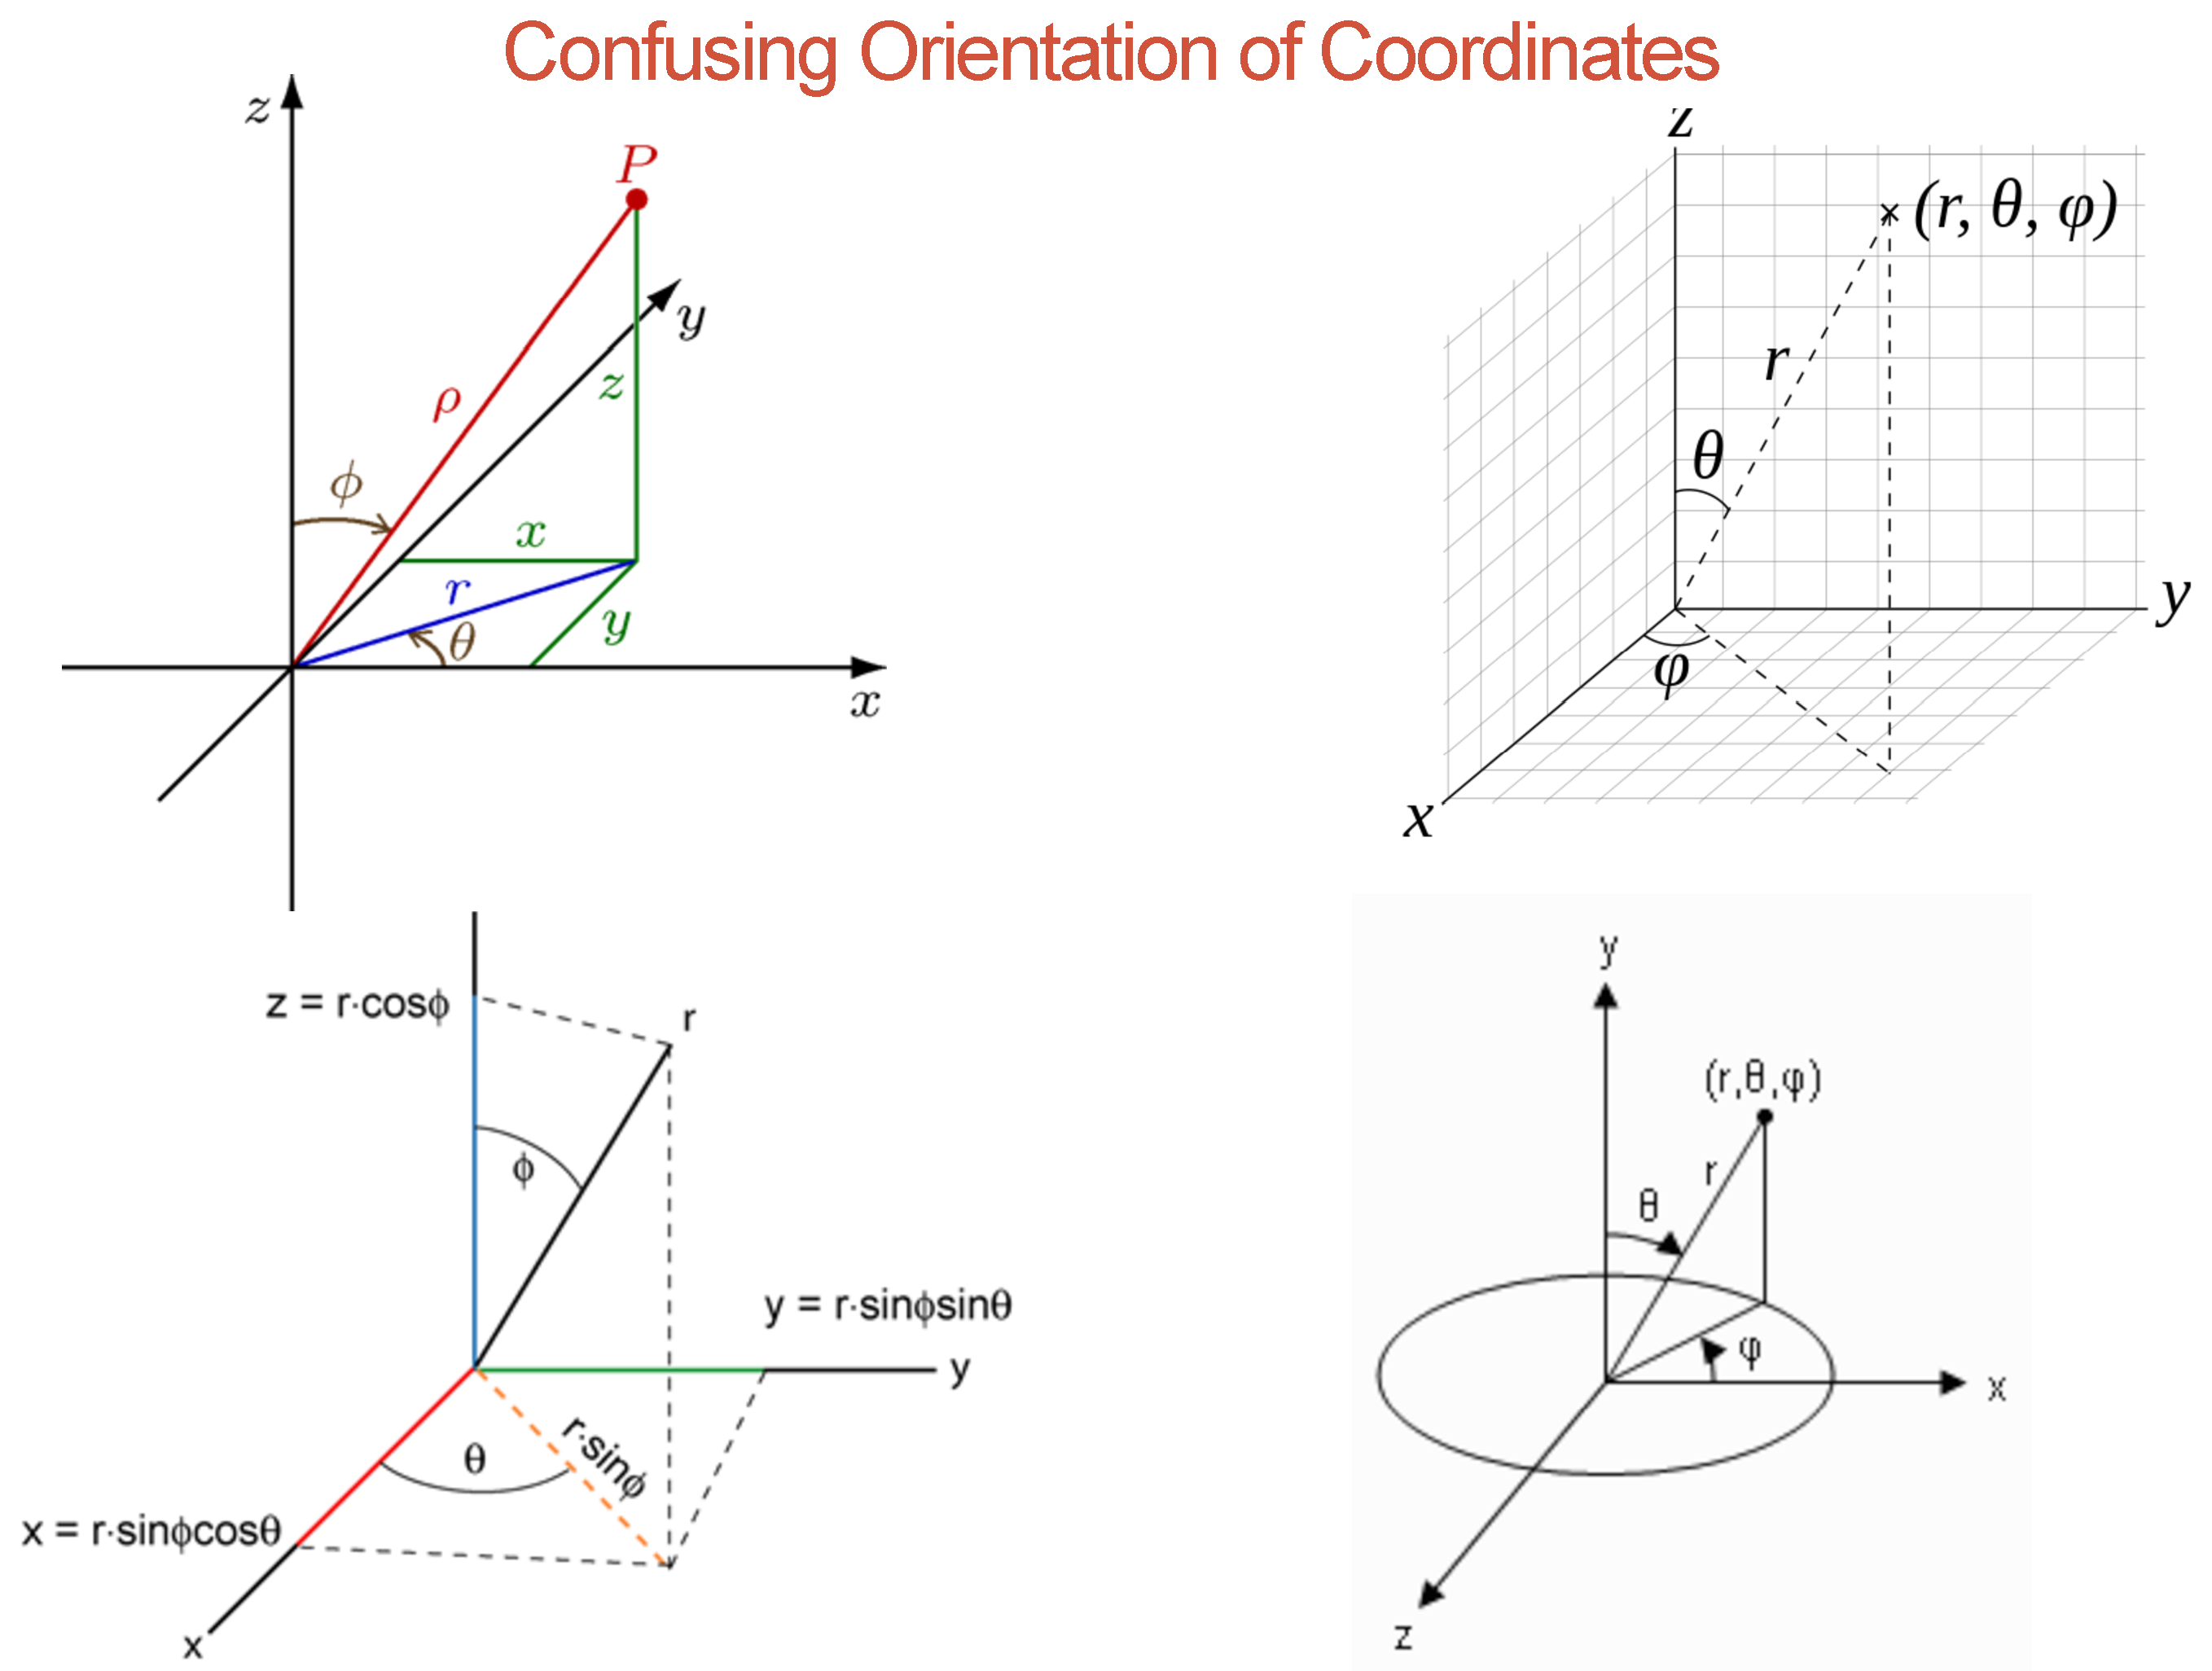
\includegraphics[width=4in]{images/pin/all-coord.png}
  \caption{Different Ways to Define Coordinate Systems} \label{all-coord}
\end{figure}
\begin{figure}[h]
  \centering
  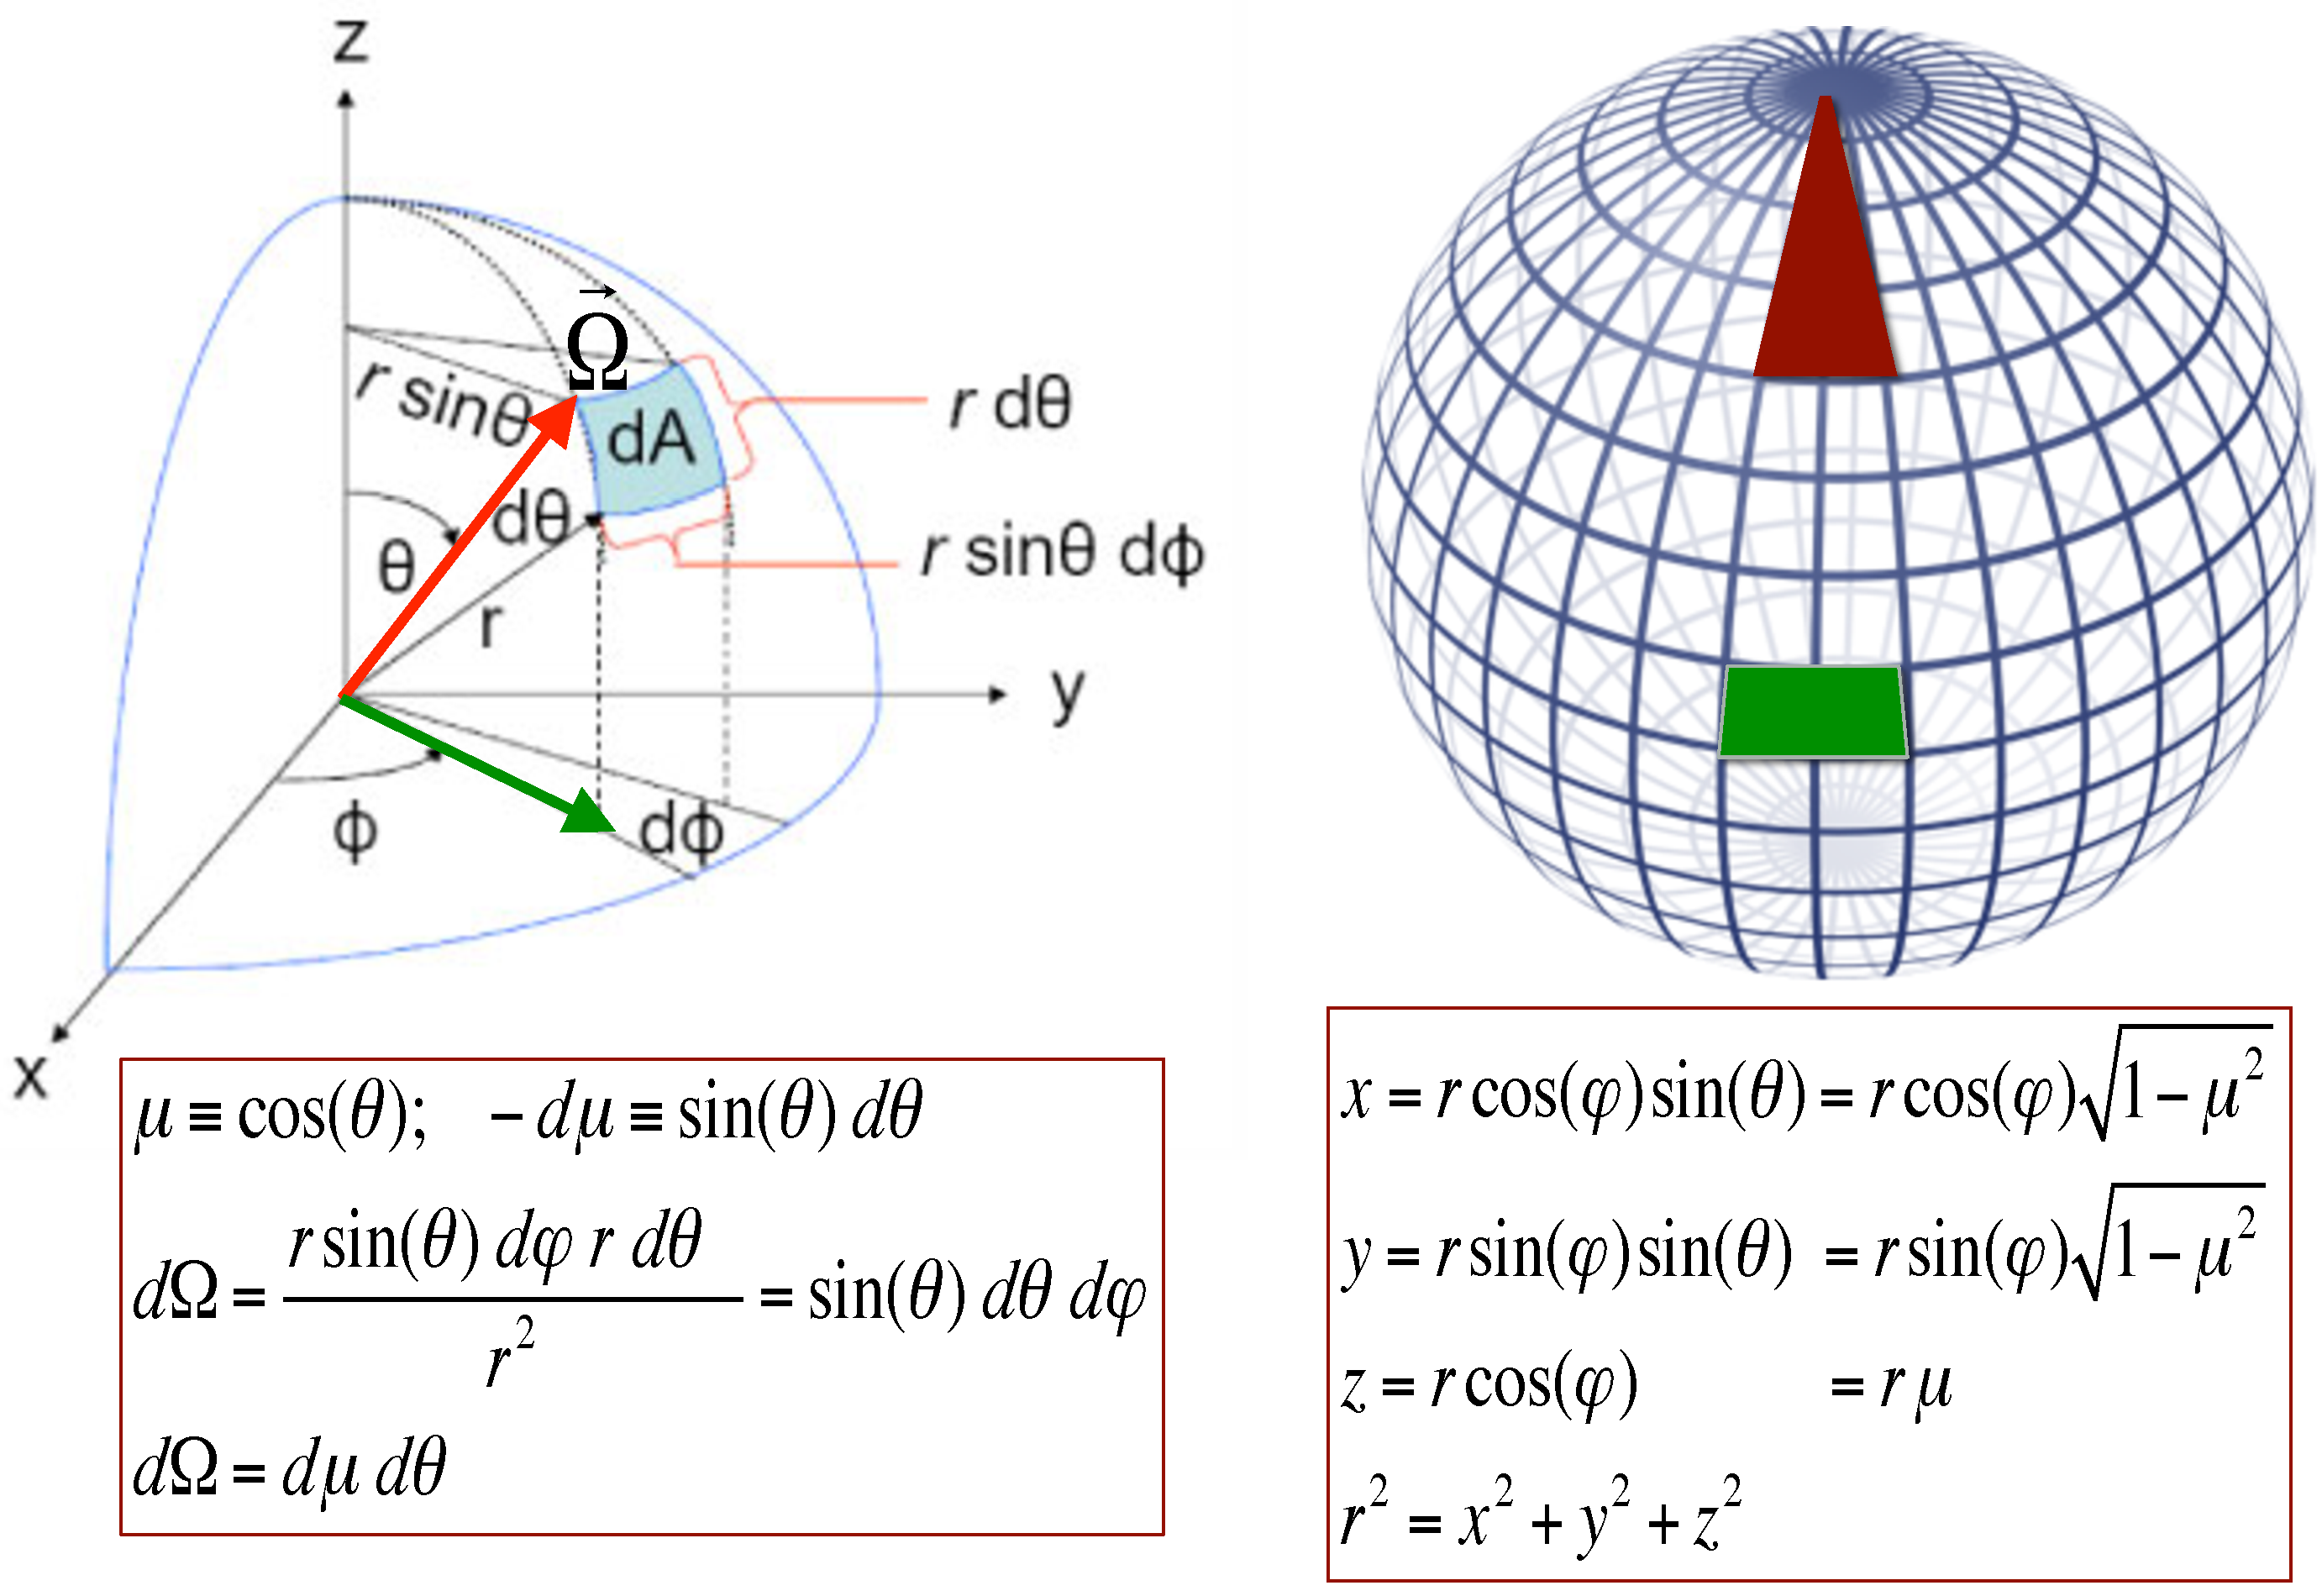
\includegraphics[width=4in]{images/pin/coord-1.png}
  \caption{Our Choice of Coordinate Systems and Area of Unit Surface} \label{coord-1}
\end{figure}


\clearpage
\topic{Infinite Slab Transport by Methods of Chords} %March 13, 2013
See Bell \& Glasstone for more details. Method of chords is kind of like MOC over a volume. 

\textbf{Basic Concept}: Method of chords takes a tube that goes through the origin, and consider where the tube contact the surface of the slab, and define the polar angle as $\theta$, the azimuthal angle as $\phi$, and the normal vector to the slab surface to be $\hat{n}$ as in Fig.~\ref{inf-plane-1}. 

\begin{figure}[h]
  \centering
  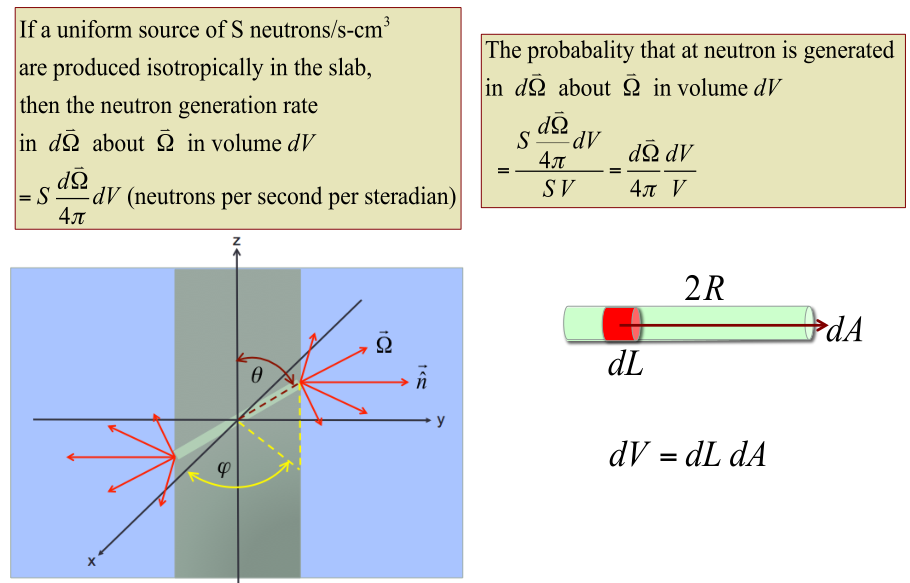
\includegraphics[width=4in]{images/pin/inf-plane-1.png}
  \caption{Setup of Infinite Slab Problem using Methods of Chords} \label{inf-plane-1}
\end{figure}
 If we assume an uniform isotropic source of $S$ neutrons/$\s\cm^2$. The probability that a neutron is generated in $\dOmega$ about $\hat{\Omega}$ in volume $\dV$ is, 
\eqn{ \frac{\dOmega}{4 \pi} \frac{\dV}{V} }
Notice the orientation of the tubes determined how many of them there are to represent the geometry as illustrated in Fig.~\ref{inf-plane-2}. 
\begin{figure}[h]
  \centering
  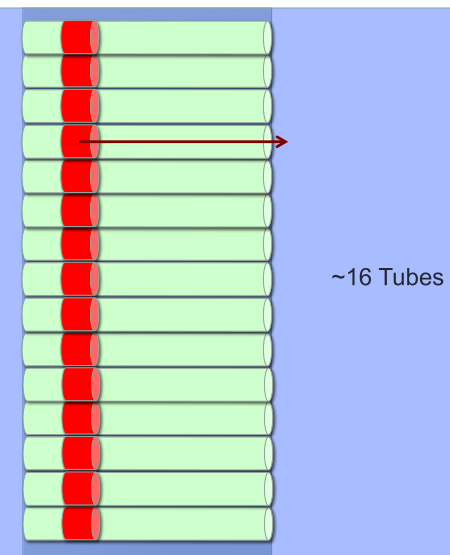
\includegraphics[width=0.31\linewidth]{images/pin/inf-plane-2.png}
  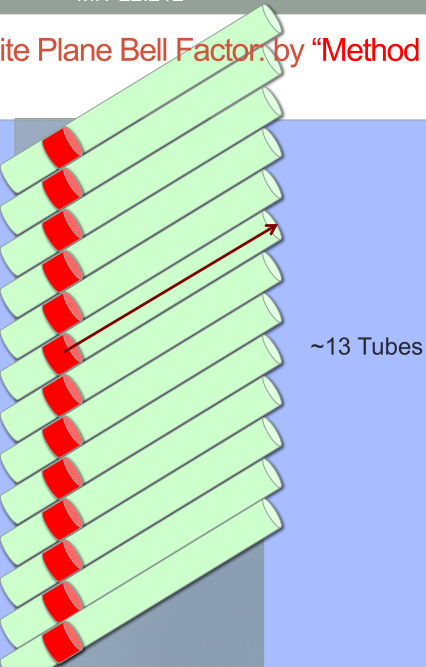
\includegraphics[width=0.31\linewidth]{images/pin/inf-plane-3.png}
  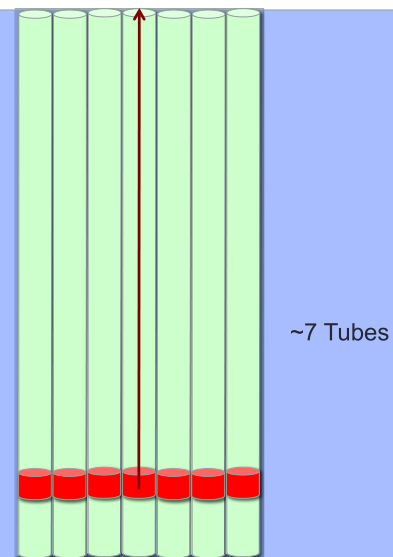
\includegraphics[width=0.31\linewidth]{images/pin/inf-plane-4.png}
  \caption{Tube Presentation in Methods of Chords} \label{inf-plane-2}
\end{figure}

\begin{figure}[h]
  \centering
  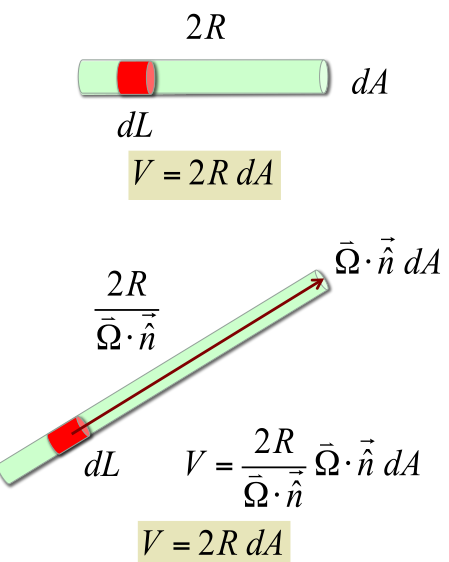
\includegraphics[width=0.45\linewidth]{images/pin/inf-plane-5.png}
  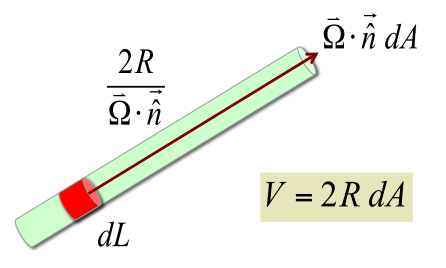
\includegraphics[width=0.45\linewidth]{images/pin/inf-plane-6.png}
  \caption{Tube Illustrations in Methods of Chords} \label{inf-plane-3}
\end{figure}



Important note: in polar angle, instead of uniformally pick $\theta$, we uniformally pick $\mu = \cos \theta$. We just sample $\Delta u /$\# polar angles. In the azimuthal angle, we sample $2\pi$/\# azimuthal angles. 


\textbf{Results}: the more polar angles and azimuthal angles we have, the better agreement we have with the Bell factor curve. 




\clearpage
\topic{Infinite Slab Transport by Direct 3D Volume Integration}
We use the finite volume approach, and basically get the same integral. 

\textbf{Results}: with 100 spatial mesh, 10 polar angles, 20 azimuthal angles we get good agreement. Notice the sensitivity on the number of spatial mesh: it takes 60 spatial meshes to get a close agreement. That is, the advantage of method of chords is that by doing math we remove 


\clearpage
\topic{Infinite Slab Transport by Monte Carlo}
We pick random $x, \mu, \phi$, find $\tau$, find $P_{FF} = 1 - e^{-\Sigma \tau}$. 



\clearpage
\topic{Infinite Cylindrical Transport by Direct Numerical Volume Integration}
Moving to cylindrical geometry, we now have four variables and need 4 integrals: $x,y, \phi, \theta$. Sensitivities: more sensitive to the azimuthal angle in cylindrical geometry; more 


For each pin, loop over all isotopes, interpolate the tables for two terms, and then multiply the corresponding $\beta$ or $1-\beta$ that only depends on Dancoff Factors. The pre-computed table stores RI as a function of background cross section, isotope type, energy. 



\clearpage
\topic{Infinite Cylindrical Transport by Monte Carlo}

\topic{Infinite Cylinder in Squre Cell Transport by Monte Carlo}
This is a simple pin cell code that treats energy dependency from Monte Carlo slowing down, and treats spatial dependency from resolving collision probabilities. Again the results generated from this model are averaged values. 

\begin{figure}[h]
  \centering
  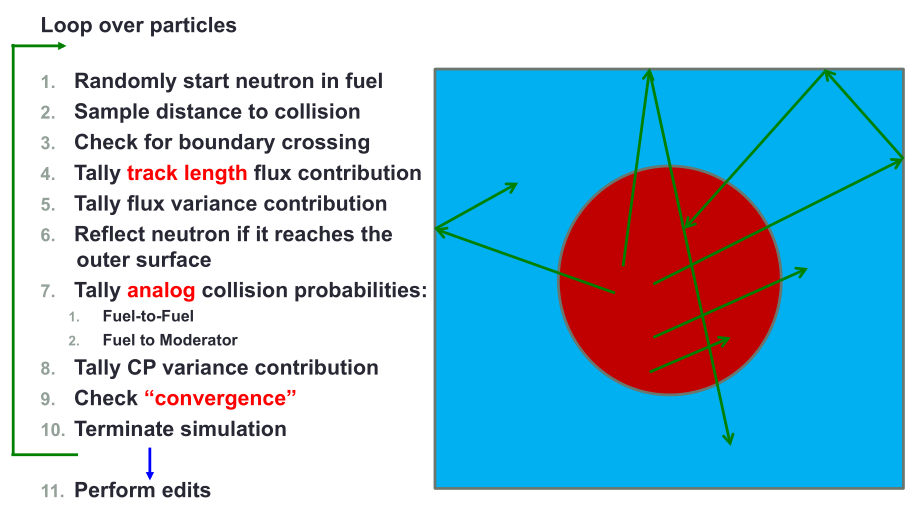
\includegraphics[width=4in]{images/pin/MC-pincell.png}
  \caption{Monte Carlo Pin Cell Algorithm}
\end{figure}

\textbf{Problem Description} (HW5 from Spring 2013 22.212):
\begin{enumerate}
\item Spatial treatment: an one-group flux calculation (one-group volume-averaged fluxes in fuel and coolant), that is, we fix the fuel absorption xs, fuel has no scattering, and fix coolant abs xs (adjust it for different cases). The reason is that we assume the separability of flux's dependency on energy and its dependency on space. 

\item Energy fine structure and a piece of the geometry treatment: Dancoff factor. We can tabulate Dancoff factors and $P_{FF}$ as a function of coolant cross sections. 

\item For this model, we do not have any IR (intermediate range) $\lambda$'s and no isotropic number densities.

\item Tracklength sampling:  let $f(x)$ be the probability of starting at $0$ and collide in $\dx$ about $x$, 
\eqn{ f(x) &= \Sigma e^{-\Sigma_t x} \dx & F(x) &= \int_0^x f(x') \dx' = 1 - e^{-\Sigma_t x} }
Then to sample a random tracklength, 
\eqn{ x &= - \frac{\ln \xi}{\Sigma_t}}
Notice the limits work out too: $-\ln(0) = \infty, -\ln(1) = 0$. 

\item Tracklength tally: tallies estimators can be incremented as each track is generated. Every neutron that ever crosses any region would contribute to the statistics, which makes it better than analog collision type.

\item Three assumptions went into this history-based statistics: central limit theorem, law of large numbers, independency. In a fixed source problem, neutrons are independent from each other, so history-based statistics are fine. 

\item \hi{History-based variance estimators cannot be incremented and squared until this history ends}:
  \eqn{ s^2 = \left( \frac{1}{N-1} \Sum_i x_i^2 \right) - \bar{x}^2} 
  History-based standard deviation of means:
  \eqn{ \sigma = \sqrt{\frac{s^2}{N-1}} }
  where sample mean is calculated from, 
  \eqn{ \bar{x} = \frac{1}{N} \Sum_i x_i }
\item Unit cell boundary conditions: 
  \begin{figure}[h]
    \centering
    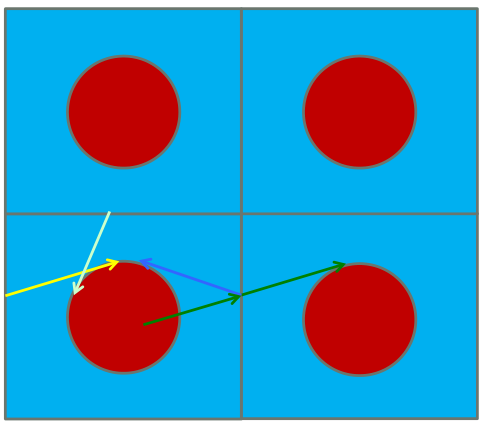
\includegraphics[width=4in]{images/pin/BC1.png}
    \caption{Pin Cell Code Boundary Conditions} \label{BC1}
  \end{figure}
  \begin{enumerate}
    \item Multiple cell typically uses natural BC as illustrated in green in Fig.~\ref{BC1}. 
    \item Reflective: illustrated in blue in Fig.~\ref{BC1}.  
    \item Opposite face periodic BC: illustrated in yellow in Fig.~\ref{BC1}. 
This BC is good for repeating geometries, especially checker-board repeating geometries the ABCD pattern in the left plot of Fig.~\ref{BC2}. For more specific geometries, full core periodic BC and quarter core mirrow BC are equivalent. 
    \item `Right-hand' rotational BC: all 1st cycle PWR are octance symmetric, then we shuffle fuels, and place the depleted fuel assemblies on the axis. 
      \begin{itemize}
      \item Our core is not diagonally symmetric, and 1/4 core rotational symmetry introduces lots of flexibility (e.g., allows us to balance reactivity along major axes instead of placing two fresh fuels next to each other). 
      \item Notice 1/4 mirros is not possible any more; instead we simulate 7 cells (as surrounded by the dark red lines in Fig.~\ref{BC2}), where these 7 cells can be arbitrary. 
      \item The advantage of keeping full nodes (instead of modeling the geometry marked by `CL'on the graph, that is, keeping 1/2 node on the axis and 1/4 on the corner) is to preserve the truncation error and thus get the same results regardless of whether we are solving quadrature, quarter or full core. 
      \end{itemize}
  \end{enumerate}
  \begin{figure}[h]
    \centering
    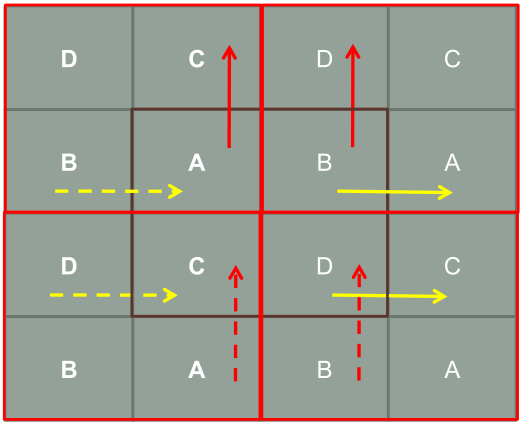
\includegraphics[width=0.45\textwidth]{images/pin/BC2.png}
    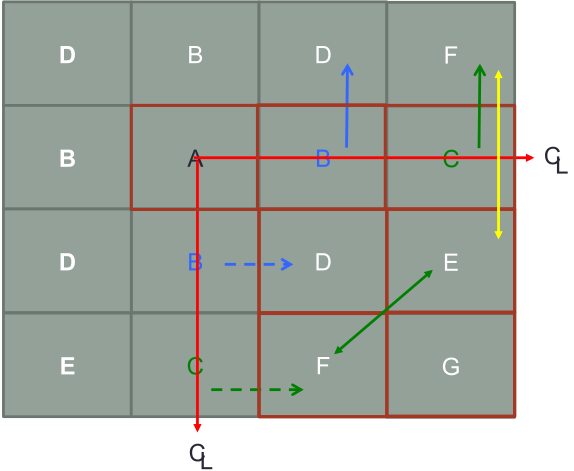
\includegraphics[width=0.45\textwidth]{images/pin/BC3.png}
    \caption{Pin Cell Code Boundary Conditions: Opposite Face Periodic and Rotational} \label{BC2}
  \end{figure}

\item $k_{\infty}$ is the number of absorption should equal to the total number of neutrons; in our case, we are losing a small portion of neutrons to the cutoff energy; we can cheat by pushing those neutrons back up. 

\item We almost always tally reaction rate or flux. Then at the end of the tallying, 
$\kinf$ and effective cross sections can be calculated from:
\eqn{ \kinf &= \frac{\bar{\nu} \Sum \Sigma_f \phi}{\Sum \Sigma_a \phi} &
\bar{\Sigma}_{xg} &= \frac{\Sum \Sigma_{xg} \phi_g}{\Sum \phi_g}}

\item Flux disadvantage factor: (flux of the fuel times fuel volume) / (flux of the moderator times moderator volume). 

\item For debugging purpose, test the following limits: compute single rod $P_{FF}$ for $\Sigma^F$ large and small; computed single rod and rod array $P_{FF}$ for thick pitch limit; compute rod array Dancoff factor for thick pitch limit, $\sigma_M = 0, \infty$. 
\end{enumerate}

\textbf{Results}: our Monte Carlo tools predict LWR parameters reasonable accurately,
\begin{enumerate}
\item $\kinf$ has a bias of about -700pcm relative to CASMO-5;
\item Reactivity (differential) effects are very accurate:
  \begin{itemize}
  \item Enrichment worth is within a couple of percent;
  \item Doppler worth is within a couple of percent;
  \item Boron worth is within about 5 percent;
  \end{itemize}
\item We should be able to use this tool to generate accurate differential reactivity effects and cross section data for simple thermal reactor lattices;
\item Remaining errors are likely due to,
  \begin{itemize}
    \item Missing thermal bound scattering models;
    \item Missing inelastic scattering;
    \item Missing unresolved resonance models;
    \item Simplified 2-region treatment, isotropic scattering;
    \item $P_{ff}$ from rational approximation, simple Dancoff factor. 
  \end{itemize}

\item Notes on flux depression factors: 
  \begin{itemize}
  \item Flux depression factor in fuel does not depend on collision rates in moderator $\Sigma_m V_m$, and it does not depend on the lattice pitch. This is from the approximation that there is an uniform source in the moderator. 

  \item Flux depression factor in moderator depends on collision rates in the moderator and on the pitch. 
  \end{itemize}
\end{enumerate}
Reference: 3.6 of Albert. \hi{LWR macroscopic down scattering xs is 0.22.} It is insensitive to enrichment. The advantage of micro is that you can interpolate on enrichment with accuracy. 



\clearpage
\topic{Special Topic: Ray Tracing using Quadratic Surfaces}
\begin{enumerate}
\item Constructive Solid Geometry(CSG): this is a common methodology used to describe 2D and 3D geometries. 2D CSG models represent primitive surfaces: planes, circles, etc. Primitives divide the universe into half-spaces. For instance, a circle divides a universe into what is inside and what is outside. Then we use union, intersection, addition, subtraction to build complex objects. 


\item Quadratic surfaces: a general quadratic surface in 2D for Cartesian coordinates is, 
  \eqn{ ax^2 + by^2 + fxy + px + qy + d &= 0 }
  Some basic planes in 2D include: 
  \begin{itemize}
    \item x-plane: $x-x_0 = 0 \Rightarrow px + d =0$. 
    \item y-plane: $y-y_0 = 0 \Rightarrow qy + d = 0$. 
    \item Arbitrary plane (plane): $px + qy + d =0$. 
    \item Circle: $(x-x_0)^2 + (y-y_0)^2 + (z-z_0)^2 - R^2  = 0 \Rightarrow x^2 + y^2 - 2x_0 x - 2y_0 y + (x_0^2 + y_0^2 - R^2) = 0$. 
  \end{itemize}

\item Ray tracing: ray tracing tracks a vector across geometry. There are three primary computations: 
  \begin{enumerate}
    \item Determine which cell the point $(x,y)$ resides in. 
    \item Determine the distance to the nearest surface. 
    \item Determine the intersection point on the nearest surface. 
  \end{enumerate}
\end{enumerate}











\clearpage
\end{document}
